\documentclass[10pt,letterpaper,twocolumn]{article}

\usepackage[letterpaper,top=0.55in,bottom=0.6in,left=0.62in,right=0.62in,columnsep=0.34in]{geometry}
\usepackage[numbers,sort&compress]{natbib}
\usepackage{amsmath}
\usepackage{booktabs}
\usepackage{graphicx}
\usepackage{mathptmx}
\usepackage{microtype}
\usepackage{xcolor}

\graphicspath{{../outputs/figures/}}

\input{../report/construction/macros}
\input{../report/construction/macros-results}

% Lightweight visible marker for the draft template. Keep this local so the
% summary can compile before the final text is written.
\providecommand{\todo}[1]{\textit{\textcolor{black!65}{[TODO: #1]}}}

\newcommand{\summarytitlemain}{Sampling Coherent Weather Fields}
\newcommand{\summarytitlesub}{From Probabilistic Foundation Models}
\newcommand{\summaryauthor}{Harvey Bermingham}
\newcommand{\summaryprogramme}{MPhil Data Intensive Science}
\newcommand{\summaryinstitution}{University of Cambridge}
\newcommand{\summarywordcount}{\todo{insert final word count}}
\newcommand{\summarylimit}{1,000 words}

\newif\ifshowwordcount
% The reference summary does not show a word-count line. REQUIREMENTS.md makes a
% front-cover word count mandatory, while the writing checklist applies that to
% both report and summary; keep this false unless Sophie / the handbook confirms
% the executive summary needs it too.
\showwordcountfalse

\setlength{\parindent}{0pt}
\setlength{\parskip}{0pt}
\raggedbottom
\pagenumbering{arabic}

\makeatletter
\renewcommand\section{\@startsection {section}{1}{\z@}%
  {1.25ex plus .2ex minus .1ex}%
  {0.45ex plus .1ex}%
  {\normalfont\normalsize\bfseries}}
\makeatother

\begin{document}

\twocolumn[
\begin{@twocolumnfalse}
\begin{center}
{\fontsize{13.2}{14.6}\selectfont\bfseries\scshape\MakeUppercase{\summarytitlemain}\par}
\vspace{0.02em}
{\fontsize{10.4}{12}\selectfont\scshape\MakeUppercase{\summarytitlesub}\par}
\vspace{0.32em}
{\fontsize{7.9}{9.4}\selectfont\scshape
\MakeUppercase{\summaryauthor}\quad\(\vert\)\quad
\MakeUppercase{\summaryprogramme}\quad\(\vert\)\quad
\MakeUppercase{\summaryinstitution}\par}
\ifshowwordcount
\vspace{0.25em}
{\fontsize{8.5}{10}\selectfont Word count: \summarywordcount \quad Limit: \summarylimit\par}
\fi
\end{center}
\vspace{0.35em}
\end{@twocolumnfalse}
]

% This is a template, not approved prose. Flesh it only after the report is
% final enough to derive from, following research_notes/writing/exec-summary.md.
% Requirements:
% - separate document, <= 1,000 words;
% - broader audience: senior managers / grant reviewers;
% - why it matters, impact, next steps;
% - numbers via macros only;
% - no predictive-skill or ensemble-calibration over-claim.

\section*{Motivation \& Scientific Justification}

Weather forecasts inform decisions across agriculture, energy, transport and emergency
planning, and recent years have repeatedly broken temperature records. Preparing for
droughts and heatwaves therefore depends not only on the most likely outcome but on how
confident that prediction is. Operational forecasts traditionally express this uncertainty by running
a physics-based model many times from perturbed starting conditions.

Machine-learning weather models now supplement this repeated simulation. Many output
a single best value at each location, which does not carry the model's uncertainty,
whilst others such as GenCast \cite{price2024gencast} generate whole ensembles of
fields. The WeatherGenerator \cite{weathergenerator}, a foundation weather model
developed at ECMWF of the same kind as AtmoRep \cite{lessig2023atmorep} and Aurora
\cite{bodnar2024aurora}, has a branch that instead outputs a Gaussian mixture at every
grid location, a blend of four weighted bell-shaped components. This means the forecast
itself carries the model's uncertainty and can hold several distinct plausible outcomes
at once. However, due to computational constraints each location's mixture is produced on
its own, and the model holds no covariance between locations. Sampling each location
independently therefore gives a noisy field unlike any real weather pattern
(Figure~\ref{fig:sum-hook}).

Many of the quantities forecasts exist to provide also belong to a whole field rather
than a single location, such as the total rainfall over a river catchment, and each
depends on how locations vary together, so it can only be drawn from a field that
could actually occur. This research supplies that missing step for the WeatherGenerator's Gaussian-mixture
branch, assembling its independently produced mixtures into one coherent field.

\begin{figure}[t]
  \centering
  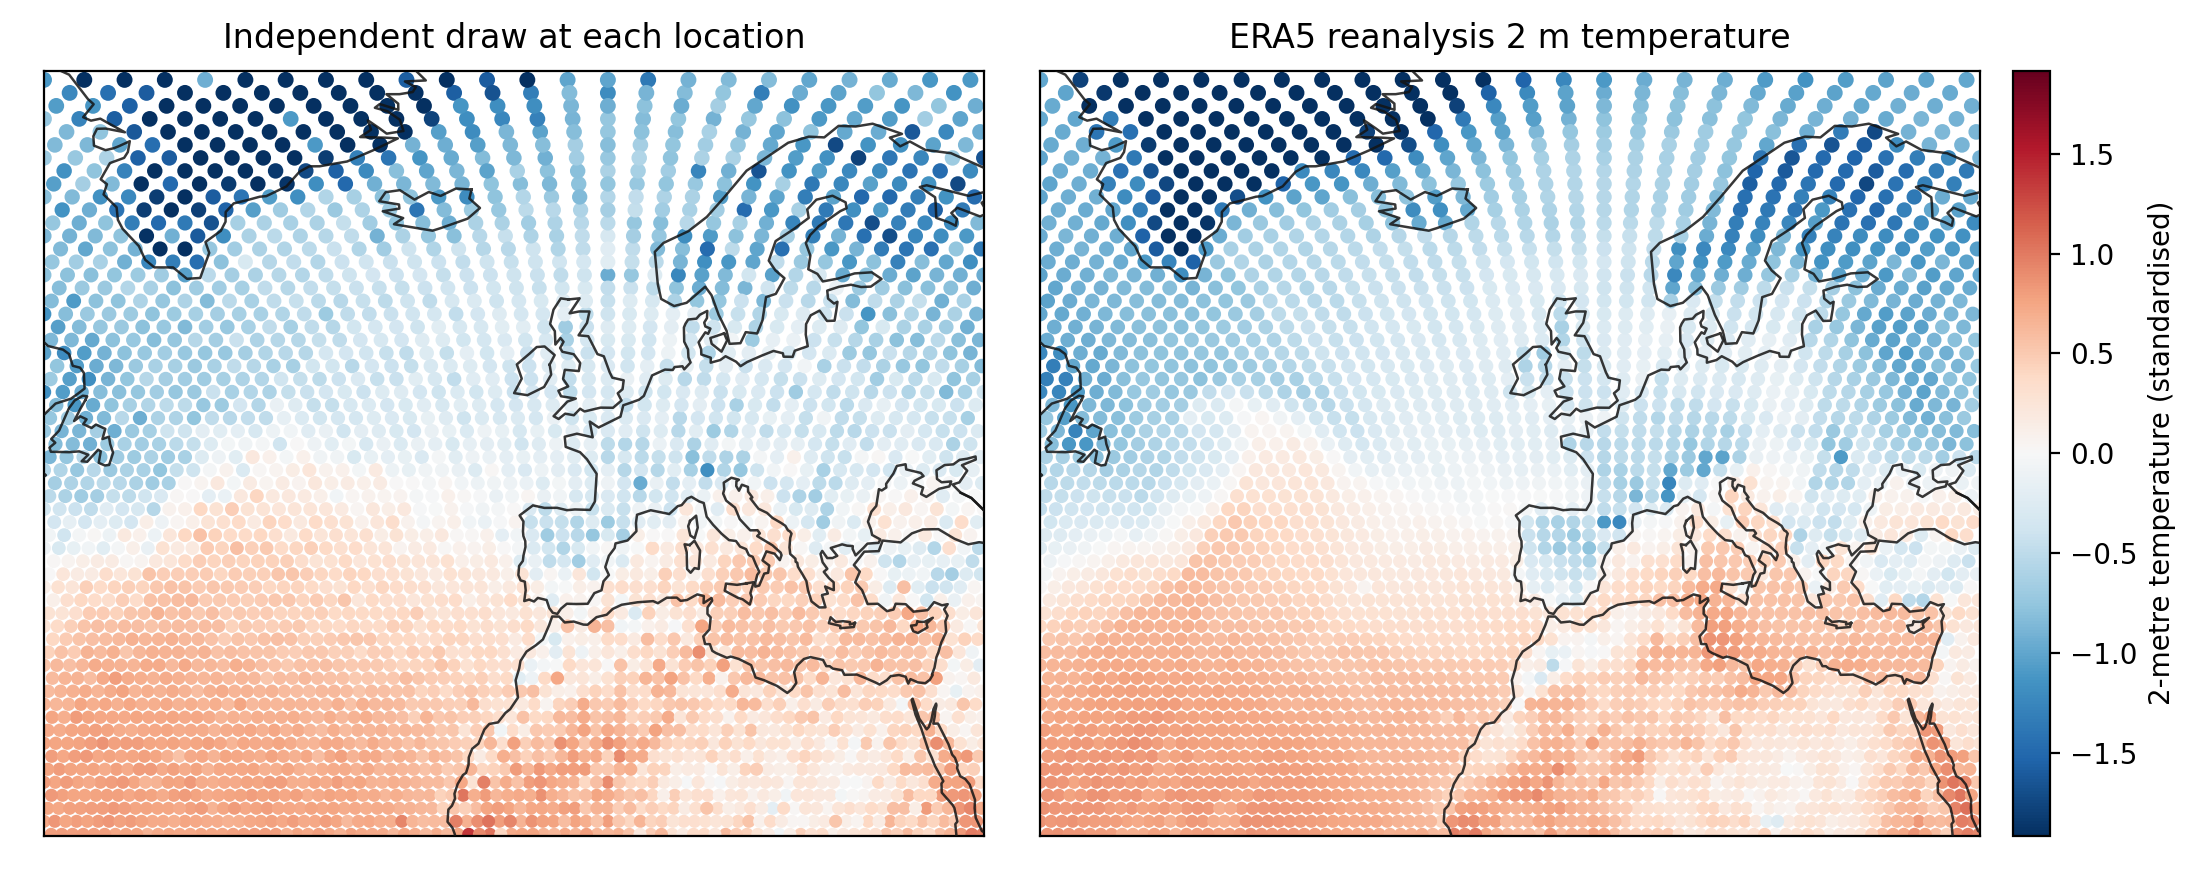
\includegraphics[width=\linewidth]{fig_hook_noise_vs_structure.png}
  \caption{A field drawn independently from each location's emitted mixture (left)
  carries fine-scale noise that no real weather field shows, whereas the ERA5
  \cite{hersbach2020era5} record of 2-metre temperature on the same grid (right) varies
  coherently across space. Each dot
  is one grid location, shown over the North Atlantic and Europe.}
  \label{fig:sum-hook}
\end{figure}

\section*{Methodology}

The sampling method, Joint MAP, chooses one value at every location by balancing two
requirements. Each
chosen value must stay plausible under its own location's mixture, and neighbouring
values must vary smoothly across the grid. The smoothness is a prior we assume and
impose on the method, not a recovery of the covariance the model discarded. The
research takes the emitted mixtures as fixed input, and it is not itself a forecasting
model and does not aim to improve forecast accuracy. The strength of the smoothing can
be varied to suit the use. For comparison it is tuned to a fixed reference, so
competing methods are judged at the same smoothness rather than any setting being
treated as the correct one.

The sampler was first exercised on a small synthetically constructed testbed whose
mixtures are specified in advance, so the coherent underlying distributions are known
and give direct context on how successfully the sampler rebuilds a field. Its independently
drawn mixture weights also make it a demanding case, with few locations holding one
dominant value. The sampler was then tested on real 48-hour temperature forecasts
across roughly forty thousand grid locations covering the globe, from
\comparisonNInits{} start dates spanning the seasons of 2023, which lies outside the
model's training period.

\section*{Key Findings}

The sampled fields were compared against several baselines, from an independent draw at
each location to a smoothed field of the single most likely values.
At the same smoothness the sampler was found to keep far more locations on values the
model itself rates plausible, with the smoothed baseline leaving \fcSmearBlurNTen{} of locations on
unlikely in-between values against the sampler's \fcSmearStar{}, roughly two and a half
times as many.

The advantage concentrates where the forecast is genuinely uncertain, at locations
whose mixture holds two distinct plausible outcomes separated by a low-probability gap,
a front arriving or not, rather than one wide overlapping spread. Within those
locations the smoothed baseline pushes \fcBimodalFracBlur{} of values into the unlikely
middle ground between the two outcomes (\bootstrapCIPct\% interval
[\fcBimodalFracBlurLo{}, \fcBimodalFracBlurHi]) against the sampler's
\fcBimodalFracMethod{} ([\fcBimodalFracMethodLo{}, \fcBimodalFracMethodHi]), an
ordering that held on all \comparisonNInits{} start dates.
Additionally, nearly every value the sampler selects sits centrally within its own
mixture, \mOneCovNinetyConvergedMean{} of locations falling in the central 90\% band
(\mOneCovNinetyConvergedLo{} to \mOneCovNinetyConvergedHi{} across start dates). This
checks each value against its own predicted distribution, not the calibration of
forecast probabilities against observed weather.

Such situations become more common as the forecast reaches further ahead. Locations
effectively certain of one value fall from \oneHotSixHourConverged{} at six hours to
\oneHotFortyEightConverged{} at 48 hours, and locations holding two well-separated
outcomes grow from \bimodalTwoSigmaSixHourConverged{} to
\bimodalTwoSigmaFortyEightConverged{}, so the conditions where the sampler is most
valuable grow with forecast range. Figure~\ref{fig:sum-maps} shows the
sampled fields beside the ERA5 record of what actually occurred.

\begin{figure}[t]
  \centering
  \includegraphics[width=\linewidth]{phase_4_fc48_14ep_step8/phase_4_region_maps.png}
  \caption{Sampled 48-hour temperature fields for one 2023 start date over the North
  Atlantic and Europe, in standardised units. Top row, the field of most likely values
  and an independent draw. Middle row, the sampler developed here (Joint MAP) beside
  the smoothed baseline at the same smoothness. Bottom row, the sampler at a lighter
  smoothing setting and the corresponding ERA5 field.}
  \label{fig:sum-maps}
\end{figure}

\section*{Impact \& Limitations}

This research provides a sampling method and evaluation architecture for
WeatherGenerator's Gaussian-mixture branch that were not previously built, and both
apply to any future model on the branch. More broadly, a coherent field is what
lets this style of forecast answer the field-level questions raised above. The step is cheap, the full evaluation completing in about
\computeAuditWallSeconds{} seconds on one processor.

This research uses only one weather variable, 2-metre temperature, one spatial
resolution and one model branch. The model
behind the mixtures is an early checkpoint that was still visibly improving when
training stopped, forecasts reach only 48 hours ahead, and the robustness check spans
the seasons of a single test year. Every comparison is made against the model's own
emitted mixtures, the only ground truth available, and whether the sampled fields match
the observed atmosphere is deliberately left to future work.

\section*{Next Steps}

The first step is to train the model out to seven to fourteen days, where the mixtures
should soften further. A preliminary seven-day run showed steady
softening but no growth yet in well-separated alternatives, though artefacts of longer forecasts are
difficult to separate from undertraining. The sampler's margin over the baselines
should grow at these ranges if the mixtures keep genuinely distinct outcomes. Sampling several
weather variables jointly, such as rain with cloud cover, would also make established
methods like Ensemble Copula Coupling \cite{schefzik2013ecc} and the Schaake shuffle
\cite{clark2004schaake} comparable.
Finer-resolution mixtures, at points a few tens of kilometres apart, should
vary more gently between neighbours, whilst weather fronts and other sharp features,
which the sampler pushes against, need preserving. Validating the fields against
observed weather is the further goal, a step towards forecasts that carry their
uncertainty through to the decisions they inform.

% Citations use only keys already present in report/construction/refs.bib. The
% file is found via BIBINPUTS (exported by the Makefile), which works both for
% latexmk's existence check and for the bibtex run inside build/.
\bibliographystyle{unsrtnat}
\bibliography{refs}

\end{document}
